\section{Time Series Decomposition}
\subsection{Business Series}
Both additive and multiplicativedecomposition models were applied to the Business series. In the additive model, the observed series is expressed as:
\[x_t = m_t + s_t + z_t\]
where $m_t$ is the trend, $s_t$ is the seasonal effect, and $z_t$ is the random component with mean zero. In the multiplicative model, the series is expressed as:
$x_t = m_t  \cdot s_t \cdot z_t$
where the seasonal effect is assumed to grow in proportion to the trend.
To determine which model is more appropriate, both decompositions were plotted and the random components were compared. 
% \begin{lstlisting}[language=R]
% decom1.add <- decompose(y1)
% decom1.mul <- decompose (y1, type="mult")

% plot(decom1.add)
% plot(decom1.mul)
% \end{lstlisting}
\begin{figure}[ht]
    \centering
    \begin{minipage}{0.49\textwidth}
        \centering
        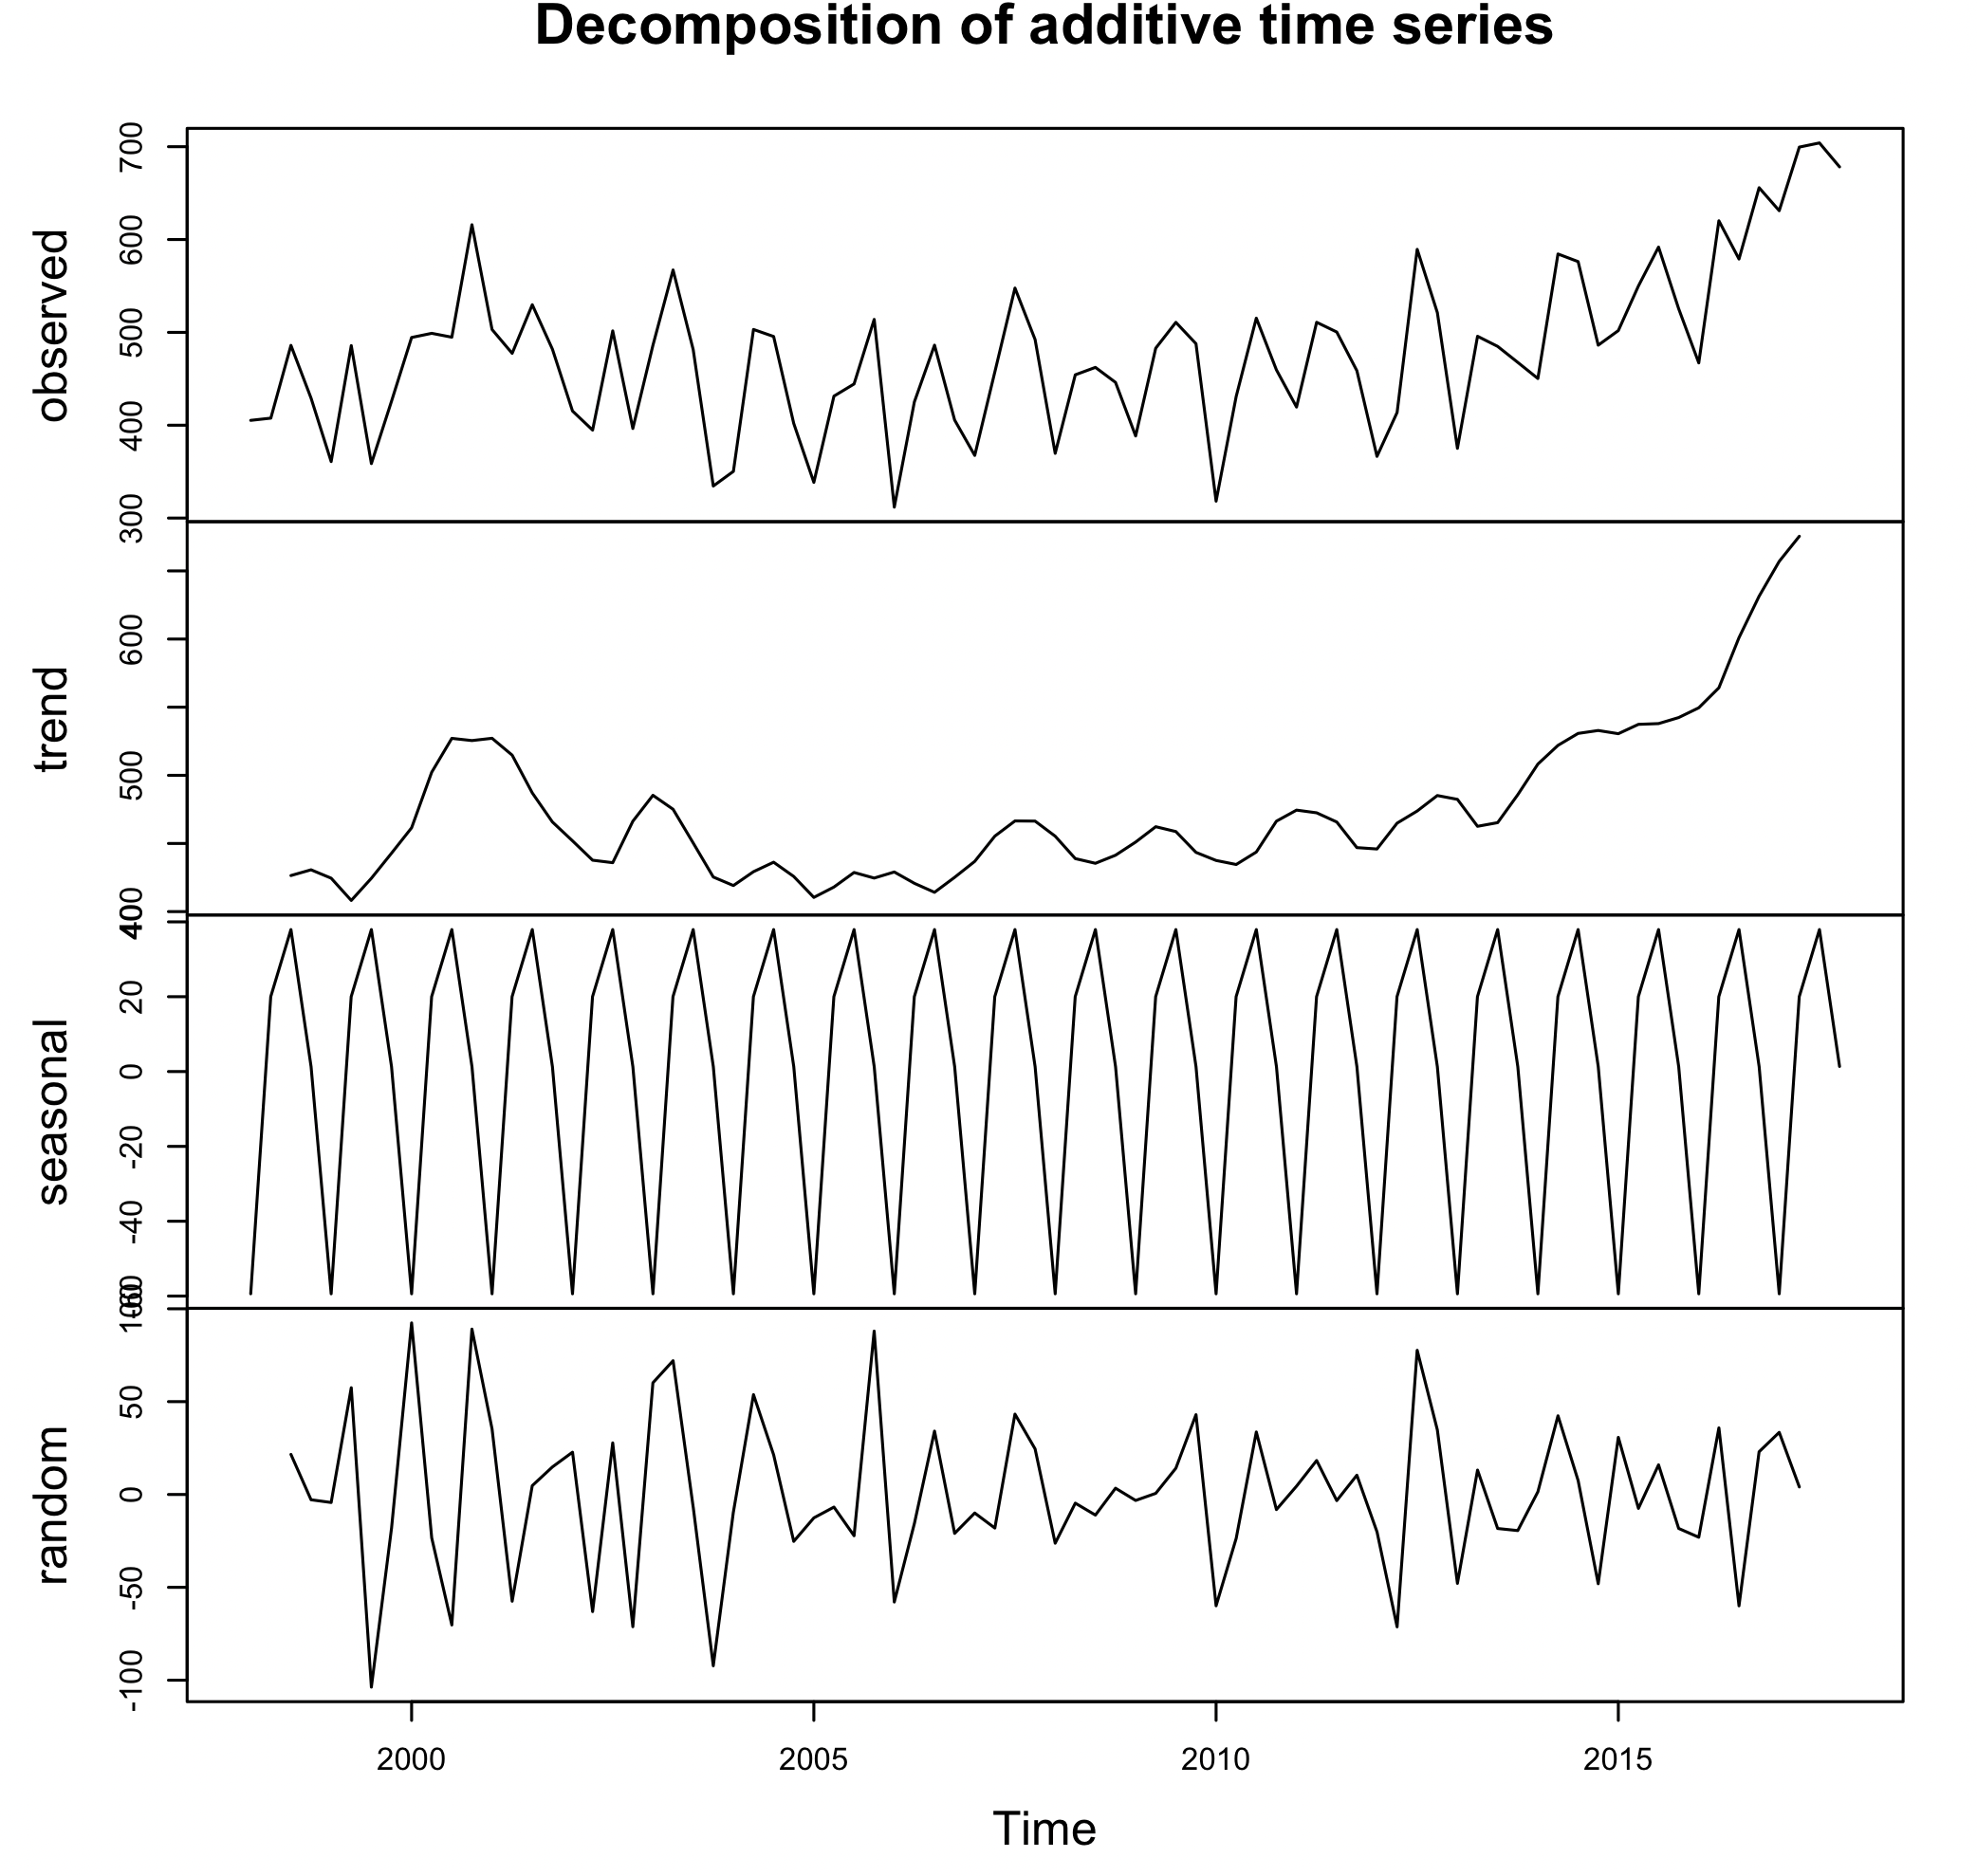
\includegraphics[width=1\linewidth]{fig/y1add.png}
        \caption{Additive decomposition}
        \label{fig:y1add}
    \end{minipage}
    \hfill
    \begin{minipage}{0.49\textwidth}
        \centering
        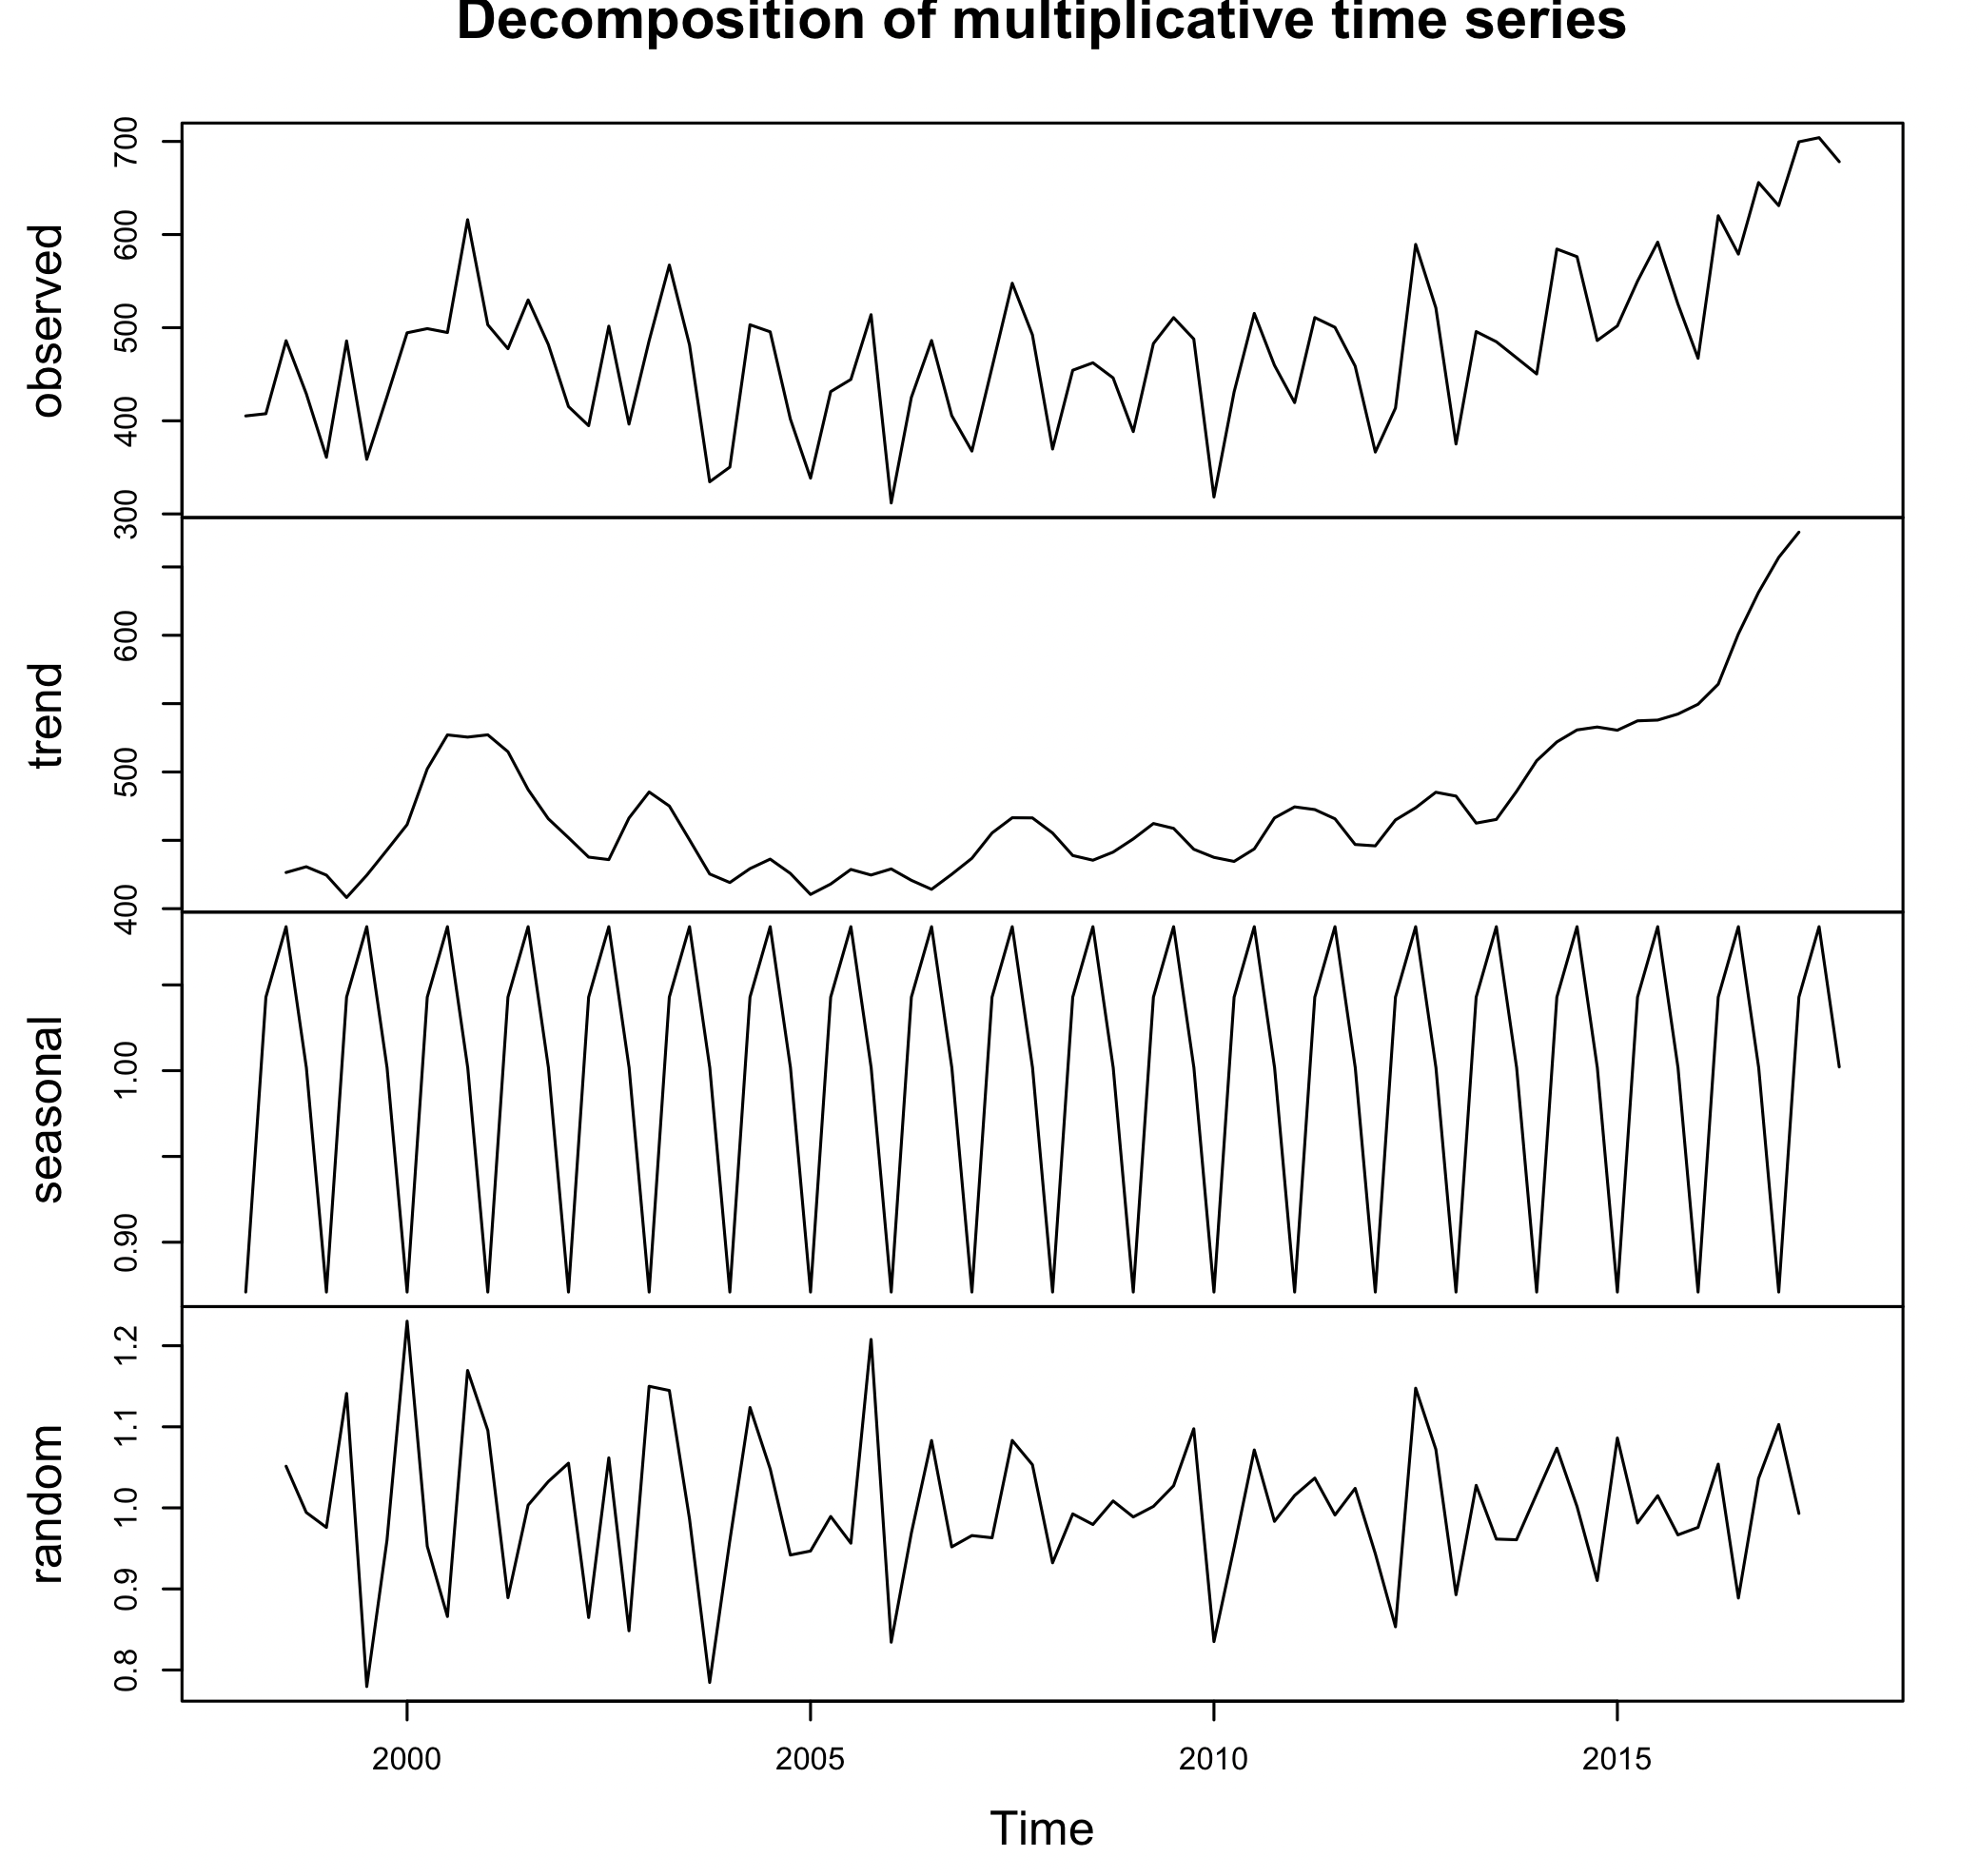
\includegraphics[width=1\linewidth]{fig/y1mul.png}
        \caption{Multiplicative decomposition}
        \label{fig:y1mul}
    \end{minipage}
\end{figure}

\noindent For the Business series, the seasonal variation does not appear to increase as the trend increases, the size of the seasonal swings remains roughly constant across the full observation period. Comparing the random components of the two models, the multiplicative residuals seems slightly more uniform as the are centered around 1.\\

\noindent Therefore we conclude that the additive decomposition model is more appropriate for the Business series, with the features:
\begin{enumerate}
    \item The trend component confirms the 2-phase behavior we observed in the time plot.
    \item The seasonal component shows a consistent repeating pattern, which is stable throughout the whole observation period.
    \item The random component shows no systematic pattern in size over time.
\end{enumerate}

\subsection{Holiday Series}

\noindent Both additive and multiplicative decomposition models were applied to the Holiday series. 
In the additive model, the observed series is expressed as:
\[
x_t = m_t + s_t + z_t
\]
where \(m_t\) represents the trend component, \(s_t\) represents the seasonal component, 
and \(z_t\) represents the random component with mean zero. 

\noindent In the multiplicative model, the series is expressed as : \[
x_t = m_t \cdot s_t \cdot z_t
\]where the seasonal variation is assumed to change proportionally with the trend.

\begin{figure}[ht]
    \centering
    \begin{minipage}{0.49\textwidth}
        \centering
        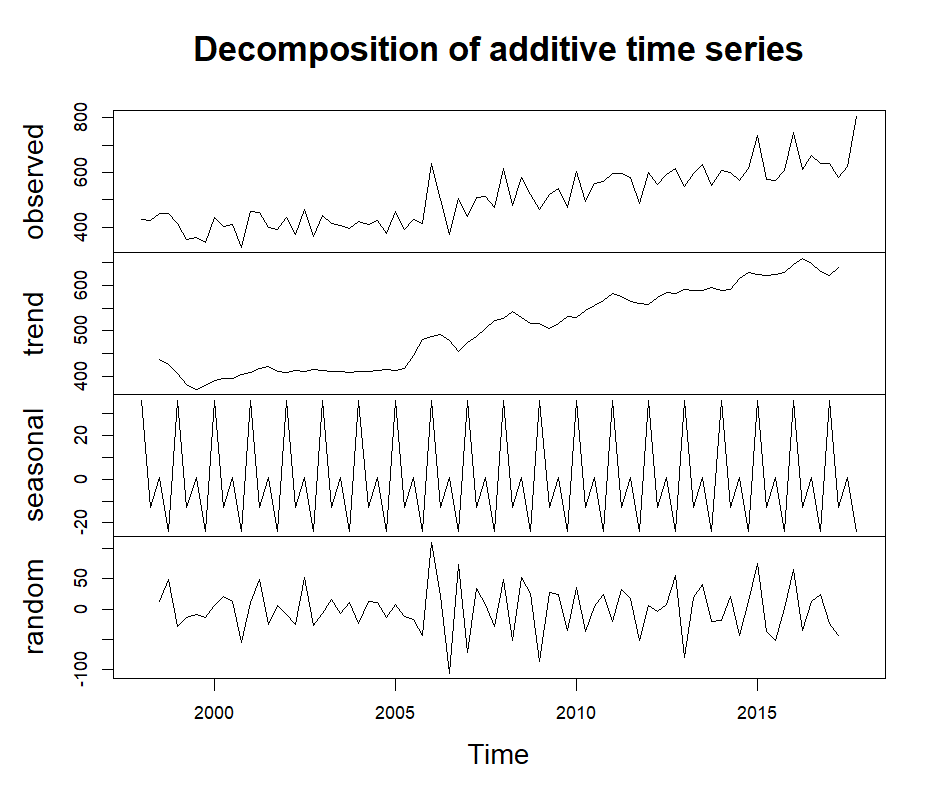
\includegraphics[width=1\linewidth]{fig/y2add.png}
            \caption{Additive decomposition}
        \label{fig:y2add}
    \end{minipage}
    \hfill
    \begin{minipage}{0.49\textwidth}
        \centering
        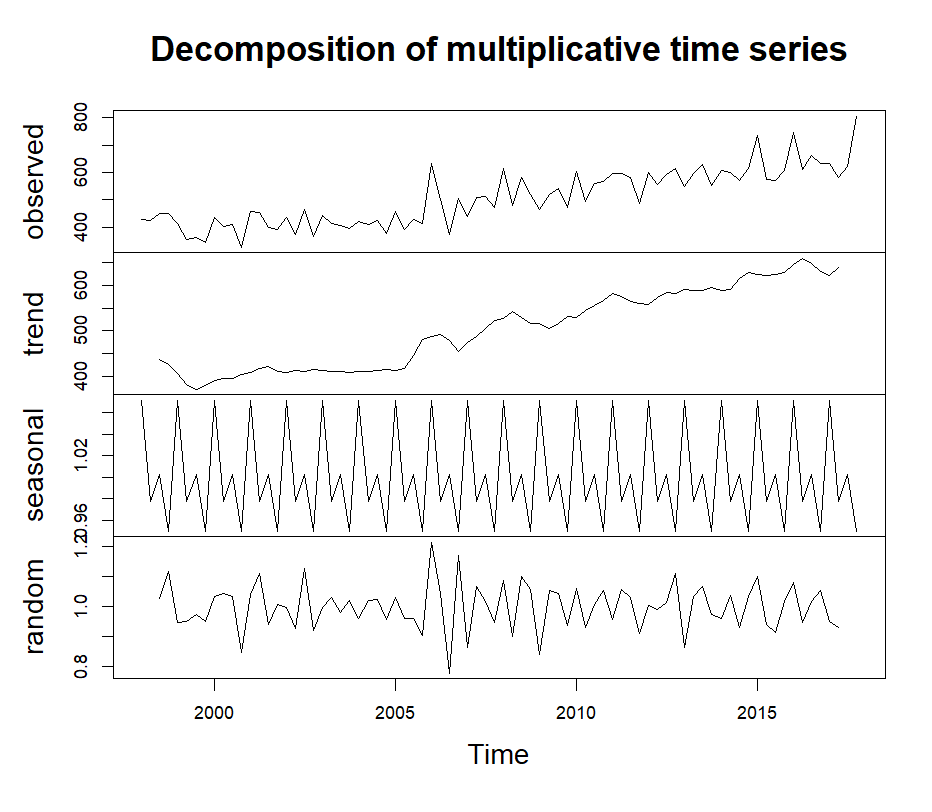
\includegraphics[width=1\linewidth]{fig/y2mul.png}
        \caption{Multiplicative decomposition}
        \label{fig:y2mul}
    \end{minipage}
\end{figure}


\noindent Figures 3 and 4 show that the additive and multiplicative decomposition results of the Holiday series. Both decomposition methods indicate the presence of trend and seasonal components. The trend component shows an overall increasing pattern, with a more noticeable increase after approximately 2006. The seasonal component exhibits a clear and consistent quarterly pattern throughout the observation period.

\noindent The seasonal variation appears to increase as the trend increases, and the size of the seasonal fluctuates over the entire observation period. Therefore, the multiplicative decomposition model is considered more appropriate for the Holiday series. The additive decomposition is included for comparison.
